\documentclass{article}
\usepackage[utf8]{inputenc}
\usepackage{hyperref}
\usepackage[margin=1in]{geometry}
\usepackage{amsmath} 
\usepackage{amssymb} 
\usepackage{indentfirst} 
\usepackage{mathrsfs}
\usepackage{verbatim}
\usepackage{hyperref}
\usepackage{bbm}
\usepackage{url}
\usepackage{graphicx,float,subfigure}
\usepackage{geometry}
\PassOptionsToPackage{hyphens}{url}
   

\title{\huge \scshape New York State Inpatients Medical Treatment and Hospital Recommender System Design}
\author{Nanqing Dong \\ \href{mailto:nd367@cornell.edu}{nd367@cornell.edu} \\ Department of Statistical Science \\ Cornell University
\and Ziyi Chen \\  \href{mailto:zc286@cornell.edu}{zc286@cornell.edu} \\ Department of Statistical Science \\ Cornell University}
\date{}

\begin{document}

\maketitle

\section{Introduction}
\indent
%We aim at recommending customized hospitals and treatments for a certain inpatient to lower mortality risk. However, whether a inpatient will survive is uncertain in advance and we have to predict.
Selection of appropriate hospitals and treatments is important for patients to recover. In this project, we aim at designing a recommender system to make customized recommendation of suitable hospitals and treatments for inpatients to lower their mortality risk, by predicting whether he/she is likely to survive with various combinations of hospitals and treatments. Such a prediction can be formulated into a binary classification problem, in which we train the classifier using the Statewide Planning and Research Cooperative System (SPARCS) Hospital Inpatient Discharges dataset [1]. This dataset has the discharge records with 39 variables of 2544731 patients. Among these variables, the ``inpatient disposition" tells us whether an inpatient survived upon discharge. \\%Table 1.\\

The rest of the paper is organized as follows: Preparation work including data preprocessing and feature engineering is shown in Section 2; The most accurate classification model is selected in Section 3; Then, in Section 4, based on the well selected model, recommender system is designed and few examples are demonstrate to test the system; The conclusion is reached in Section 5.

\section{Data Preparation}
\subsection{Data Preprocessing}
Since there are 100130 patients with missing values, which is only 3.93\% of the total number 2544731, we directly delete these samples for simplicity. In addition, the remaining number of samples is still huge compared with the number of variables, so it is not likely to overfit. Therefore, simply deleting samples with missing values is reasonable for this big dataset.\\

\subsection{Feature Engineering}
\subsubsection{Feature Selection}
The prediction of death or survival and the subsequent recommendation of hospitals and treatments can be typically conducted after preliminary diagnosis and before treatments. For example, it is normal for a patient to have preliminary diagnosis in a local clinic, and if the patient is diagnosed with a serious disease that cannot be tackled by the clinic, the clinic can recommend qualified hospitals and then the doctors select proper treatments. Hence, we delete the irrelevant features and the features that cannot be acquired upon preliminary diagnosis. The information of some typical features and the reason to select or deselect them is shown in Table 1.\\
\begin{figure}[H]
\begin{center}
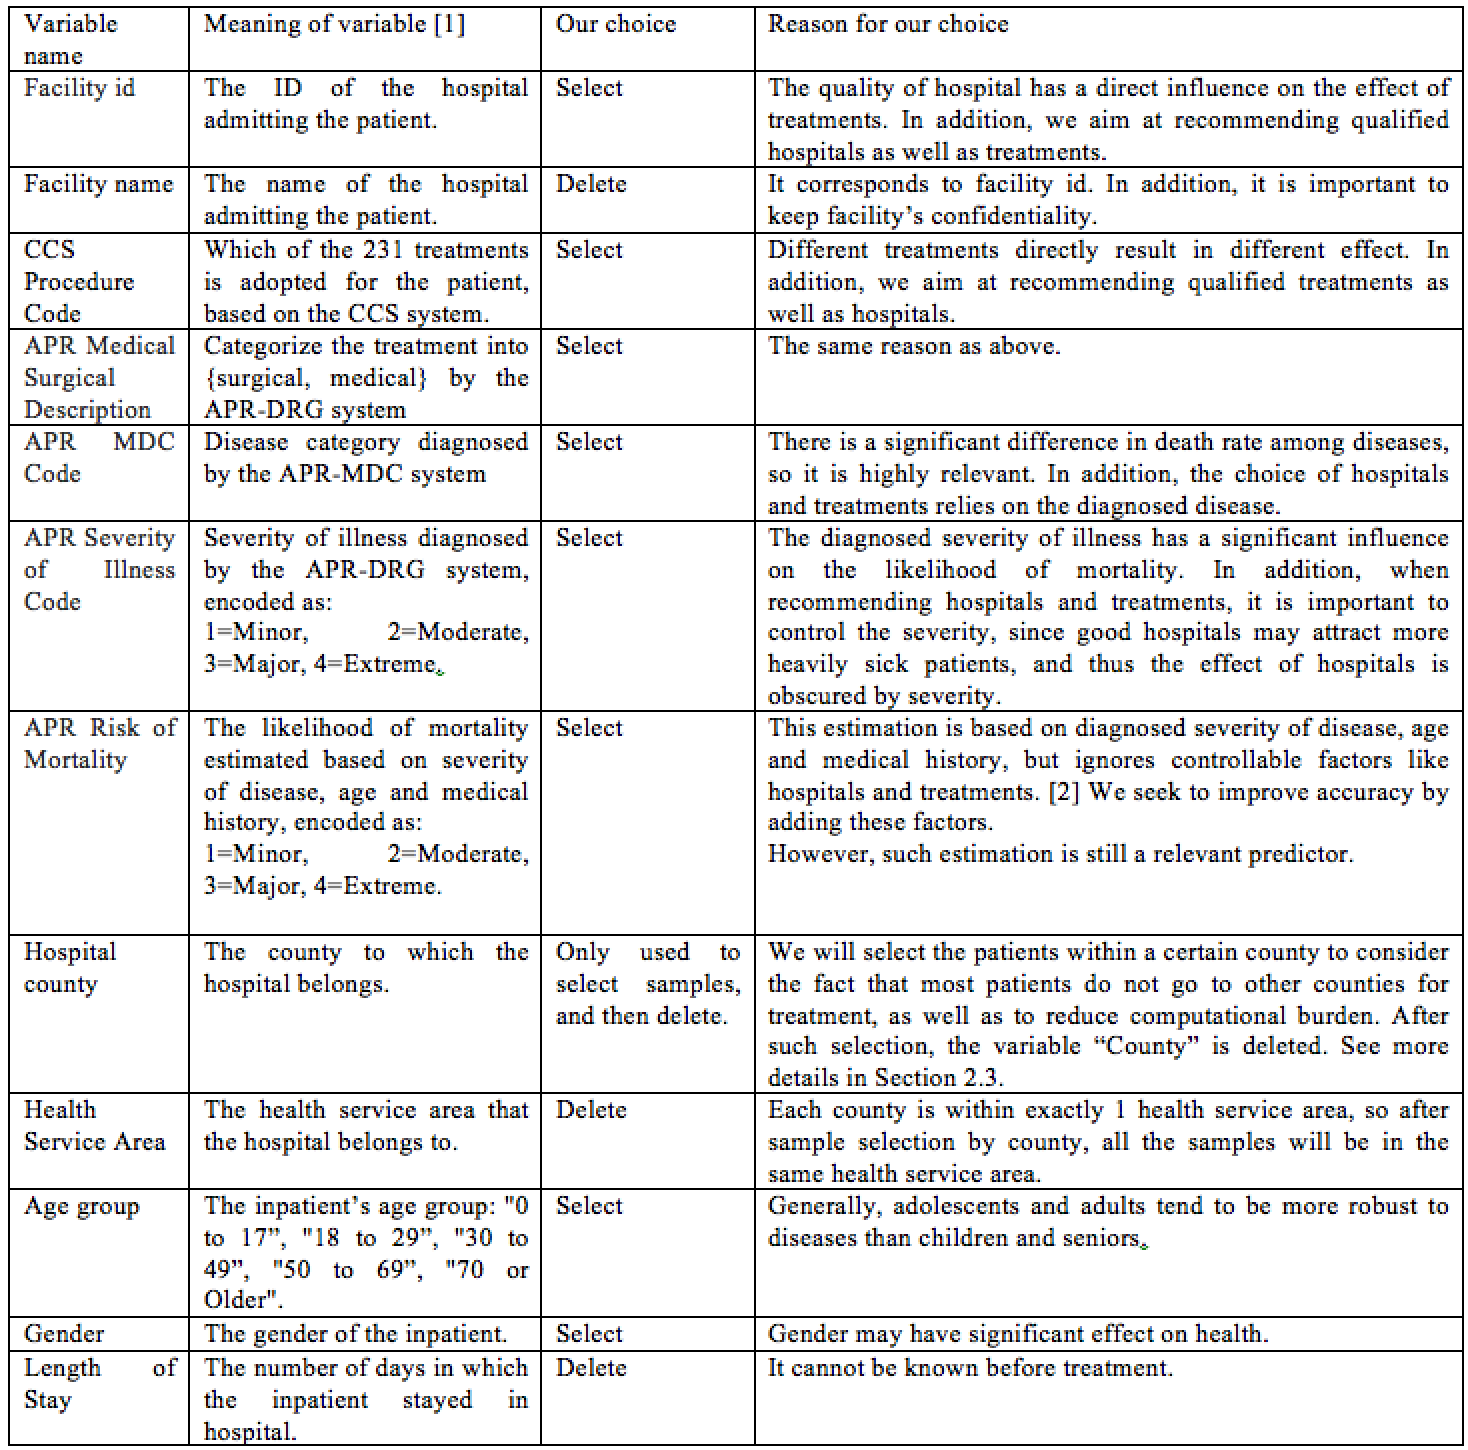
\includegraphics[width=5.0in]{table1_variable_information.png}
%\caption{Table 1: The 16 categorical predictors. \label{The 16 categorical predictors}}
\end{center}
\end{figure}
\centerline
{Table 1: Information about some typical features [1]}

\subsubsection{Feature Recategorization}

The variable ``inpatient disposition" gives the state of the inpatients upon discharge.The variable was relabelled into "Died in hospital" and "Not died in hospital" [3].\\

\subsubsection{Feature Transformation}\\
After feature selection, all the features are categorical, so we can adopt \textbf{one-hot encoding} to facilitate the classification.

\subsection{Sample Selection}
One of the biggest challenges is the high-dimension problem. The number of observations and features are both large. A single run to fit a non-parametric model may take 3 days on a 8-core computer and there is also a memory problem in matrix computation.\\

\subsubsection{Regionalization}
It is reasonable to customized the system to each county based on the fact that most patients went to local hospitals to reduce time and financial cost. In this paper, Queens, a county in New York City was selected,which has 202660 observations in the dataset.\\

\subsubsection{Representative Sampling}
In Queens, there are only 4297 died patients, which is only $2.12\%$ of the sample. Such imbalance in the 2 classes will probably result in a bias to the survived patients for the binary classification problem. In addition, variables like ``CCS Procedure Code" (Code of the treatments) has 226 values, which results large dimensionality. To solve the 2 problems, 20 values of ``CCS Procedure Code" (i. e., 20 treatments) with the highest death rate were selected to make a prototype.The proportion of died patients increased to 0.193251, and the size of the data decreased $11498\times 14$, which is easy to demonstrate here.

\section{Model Selection}
\subsection{Binary Classification}
The prediction on whether or not patients will die in the hospital is identified as a binary classification problem. In this project and following contents, "\textbf{1}" stands for "Died in hospital" and "\textbf{0}" stands for "Not died in hospital". The goal of model selection is to select a model which will have the highest prediction accuracy.

\subsubsection{F-measure}
At the first thought, test error rate was chosen as the measure for test accuracy. 
$$ \[{\rm test~error~rate = \frac{{\# misclassified~test~samples}}{{\# test~samples}}}\]
$$

However, considering the data is unbalanced, a model predicts all "\textbf{0}" will have the highest prediction accuracy. While, the predictive power for "\textbf{1}" is considered more important in this problem. So F-measure was introduced for this project.  F-measure considers both the precision and the recall of the test to compute the score: precision is the number of correct positive results divided by the number of all positive results, and recall is the number of correct positive results divided by the number of positive results that should have been returned. The $F_1$ score can be interpreted as a weighted average of the precision and recall, where an $F_1$ score reaches its best value at 1 and worst at 0.
$$ F_1 = \frac{2 * precision * recall}{precision + recall}$$
$$ precision = \frac{TP}{TP + FP}, \  recall = \frac{TP}{TP + FN}$$

\subsubsection{Naive Bayes}

\subsubsection{Logistic Regression}
Logistic Regression[5] is a special case of the  generalized linear model and thus analogous to linear regression. It has loss function:
$l_{logistic}(x,y;w) = log(1 + exp(-yw^Tx)) $.

\subsubsection{Support Vector Machines}
A Support Vector Machine (SVM)[6] is a discriminative classifier formally defined by a separating hyperplane. In other words, given labeled training data, the algorithm outputs an optimal hyperplane which categorizes new examples. \\

SVM is a relative large system for classification, the hyperparameters that were tuned are list below:\\
\textbf{C}: penalty parameter of the error term. \\
\textbf{kernel function}: linear, polynomial, sigmoid, rbf(Gaussian radial basis)\\
\textbf{class weight}: add different weight to classes to handle unbalanced problem.\\
\textbf{loss function}: hinge[5], squared hinge

\subsubsection{Random Forest}
Random forest[6] is an ensemble learning method for classification. Different classification trees are built randomly with different number of features.Each tree gives a classification, and we say the tree "votes" for that class. The forest chooses the classification having the most votes (over all the trees in the forest). \\

The hyperparameters that were tuned are list below:\\
\textbf{number of trees}: the number of trees in the forest\\
\textbf{max number of features in each tree}: $\sqrt{n}$, $log_2{n}$, $n$ (n = number of features)\\
\textbf{class weight}: add different weight to classes to handle unbalanced problem.

\subsubsection{Gradient Boosting}
Gradient boosting[7] is a machine learning technique for classification problems, which produces a prediction model in the form of an ensemble of decision trees.\\

The hyperparameters that were tuned are list below:\\
\textbf{number of boosting stages}: a large number usually results in better performance.\\
\textbf{max number of features in each tree}: $\sqrt{n}$, $log_2{n}$, $n$ (n = number of features)\\
\textbf{class weight}: add different weight to classes to handle unbalanced problem.

\subsubsection{Neural Network}
A multi-layer perceptron network[8] was trained to introduce the idea of deep learning as a comparison for other supervised learning methods.\\
\\
The hyperparameters that were tuned are list below:\\
\textbf{number of hidden layers}\\
\textbf{activation}: identity, logistic, tanh, relu(rectified linear unit function, returns f(x) = max(0, x))\\
\textbf{alpha}: $l_2$ penalty (regularization term) parameter\\
\textbf{learning rate}: constant, inverse scaling, adaptive\\

\subsection{Regularization and Shrinkage}
Two regularizer were employed here which were LASSO and Ridge to avoid overfitting. Since the data matrix is sparse, LASSO maybe a good choice and the test result aligned with prior assumption.

\subsubsection{LASSO($l_1$)}
\noindent $l_1$ regularizer[5]:
$$r(w) = \lambda \sum_{i=1}^{n} |w_i|$$
minimize $$  \sum_{i=1}^{n} (y_i - w^Tx_i)^2 + \sum_{i=1}^{n} |w_i|$$

\subsubsection{Ridge($l_2$)[5]}
\noindent $l_2$ regularizer:
$$r(w) = \lambda \sum_{i=1}^{n} w_i^2$$
minimize $$  \sum_{i=1}^{n} (y_i - w^Tx_i)^2 + \sum_{i=1}^{n} w_i^2$$

\subsection{Validation}
\subsubsection{Cross-Validation}
The original data set were split into train data, validation data and test data with a ratio 8:1:1. A random seed was set to keep the result reproducible.
The train data was used to train the classifier. The validation was used to tune the hyperparamter. The test data was used to measure the overall performance. The reason for doing this is because when tuning hyperparameters by cross-validation, the information of validation set was also incorporated in the model, so there is a chance for overfitting. Thus, an independent set, test data was needed to measure the predictiev power.

\subsubsection{Bootstrap and Confidence Intervals}
Since the data was large and non-parametric models like SVM, Gradient Boosting and Neural Network were applied, the computational cost for these models were quite large, a single run on partial data may take hours to days. Bootstrap as a common resampling method played an important role in the project. Oversampling and undersampling Bootstrap were both used to solve both unbalanced data problem and time complexity problem. In addition, confidence intervals for F-1 scores were calculated by boostrapping on randomly splitted train data.

\subsection{Result}
\subsubsection{Result Presentation}
Some representative models with tuned hyperparameters and their F-1 score are listed below. Each model in the table are the optimal models with the highest F-1 in its hyperparameter combinations.\\
\begin{center} 
    \begin{tabular}{|c|c|c|c|c|c|c|c|} 
       \hline 
       Classifier & F1 score on the & F1 score on the\\
       & validation dataset & test dataset\\
       \hline
       Logistic Regression 1$^1$ & 52.50\% &56.26\% \\
       \hline
       Logistic Regression 2$^2$ & 52.62\% & 56.48\% \\
       \hline
       Linear SVM 1$^3$ & 51.30\% & 56.36\%\\
       \hline
       Linear SVM 2$^4$ & 52.54\% &56.06\% \\
       \hline
       Linear SVM 3$^5$ & 52.47\% &55.98\%\\
       \hline
       Nonlinear SVM$^6$ & 54.13\%&57.77\%\\
       \hline
       Random Forest$^7$ & 37.72\%&\\
%       \hline
%       Gradient Boosting 1$^8$ &29.94\%&\\
%       \hline
%       Gradient Boosting 2$^9$ &31.02\%&\\
%       \hline
%       Gradient Boosting 3$^{10}$& 32.80\%&\\
       \hline
       Gradient Boosting$^{8}$& 33.78\%&\\
       \hline
       Neural Network $^{9}$ &25.84\%&\\
       \hline
       Naive Bayes &49.83\%&55.16\%\\
       \hline
    \end{tabular} 
\end{center}
\centerline
{Table 2: F1 scores for each classifier. [5]}
\centerline
{\small $^1$Logistic Regression 1: $l_2$ regularizer, C=0.061, with weighted samples}
\centerline
{\small $^2$Logistic Regression 2: $l_1$ regularizer, C=0.175, with weighted samples}
\centerline
{\small $^3$Linear SVM 1: Hinge loss, $l_2$ regularizer, C=0.001}
\centerline
{\small $^4$Linear SVM 2: Squared hinge loss, $l_1$ regularizer, C=50}
\centerline
{\small $^5$Linear SVM 3: Squared hinge loss, $l_2$ regularizer, C=1}
\centerline
{\small $^6$Nonlinear SVM: Guassian Kernel, Hinge loss, C=137}
\centerline
{\small $^7$Random Forest: number of trees=100}
%\centerline
%{\small $^8$Gradient Boosting 1: number of boosting stages=5000}
%\centerline
%{\small $^9$Gradient Boosting 2: number of boosting stages=10000}
%\centerline
%{\small $^{10}$Gradient Boosting 3: number of boosting stages=50000}
\centerline
{\small $^{8}$Gradient Boosting: number of boosting stages=100000}
\centerline
{\small $^{9}$Neural Network: number of hidden layers=100, logistic activation function, adaptive learning rate, $\alpha=0.001$}


\subsubsection{Result Analysis}
The heuristics for selecting the optimal model considers two factors:1) F1-score 2) time complexity. After comparing the validation F-1 score, Random Forest and Neural Network are filtered out. The reason assumed here is that the data matrix is quite sparse, more $70\%$ of the features have the value \textbf{0}. So the random forest method may fail, because there is a high chance that the randomly selected features may omitting the important features. Opposite to the original hypothesis,the neural network failed. The result of network was unstable, because both of random initiation and characteristics of the data matrix. Since deep learning is an advanced topic, more analysis may required to explain why neural network failed for this project.\\

SVM was chosen as the final model. We conclude that the data matrix is not separable in high-dimension space, so SVM's error tolerance mechanism can outperform other models. There is one thing worth mentioning here that even gradient boosting has a relative poor performance in either predictive power and time consuming. But it is the only models has a strictly increasing relationship with numeric hyperparameter. Some future research maybe conducted on this approach.\\
\begin{figure}[H]
\begin{center}
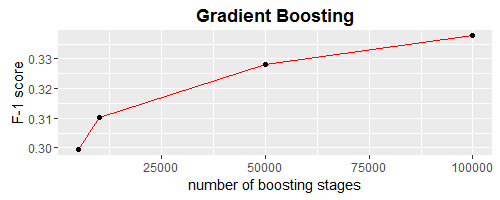
\includegraphics[width=5.0in]{boosting.png}
\caption{The F1 score of the gradient boosting with different numbers of boosting stages.}%\label{The 16 categorical predictors}}
\end{center}
\end{figure}
%\centerline
%{Figure 1: The F1 score of the gradient boosting with different numbers of boosting stages.}

\section{Recommender System Design}
\subsection{The Mechanism of the Recommender System}
\indent
The main idea of recommendation for a certain inpatient is to try all the combinations of hospitals and treatments while controlling other variables fixed. Hence, each such combination corresponds to an input vector, which can be seen as test sample. on which prediction is to be made by a well-trained SVM with Guassian Kernel, hinge loss and penalty parameter C = 137. This model and hyperparameters are chosen for recommendation because it has the highest F1 score on the test data, as shown in Section 3. In addition, the probability of death given an input $x$, i. e. , $\Pr(\textbf{1}|x)$, can be computed by SVM with Guassian Kernel. The lower probability of death means a more qualified combination for this specific patient. Therefore, we can rank all the combinations by a decreasing sequence of the probability of death.\\

\subsection{Recommendation Demo}
\indent
In this demo, select a typical patient is selected to test the robustness of the system.\\

In the Queens, among the patients whose MDC=18, severity=risk=``extreme" (The 18th disease Infectious and Parasitic Diseases, with both the highest severity level and estimated mortality risk by the APR-DRG system), there are 710 ``\textbf{1}s and 1039 ``\textbf{0}s. 5 died patients were selected to see whether this recommender system can improve their likelihood of survival by advising them to choose suitable hospitals and treatments before they died. To make the recommendation specific and more accurate for this particular serious disease, the selected SVM model is trained on the other patients whose MDC=18,  severity=risk=``extreme". For each of the 5 died patients, we generate the design matrix as the test dataset by listing all the combinations of variables ``Facility id" (Hospital ID), ``CCS Procedure Code" (Code of the 226 treatments) and ``APR Medical Surgical Description" (Categorize the treatment as medical or surgical.) while keeping the values of the other variables the same as the patient. Then, the prediction gives the probability of death for each test sample, i. e., each combination of hospitals and treatments, which is used for ranking and recommendation.\\

\subsection{Result Presentation}
\indent
As a specific example, one of the 5 patients died after receiving surgical method and treatment 34 in hospital 1626. All the possible combinations of the hospitals and treatments were sorted in decreasing sequence of the predictive 
$\log \Pr(\textbf{1})$ (log probability of death) and thus in increasing sequence of the predictive $\log \Pr(\textbf{0})$ (log probability of survival), and listed some predicted best and worst combinations in Table 3. To test the recommendation, for each combination of hospitals and treatments, all the patients with MDC=18, severity=risk=``extreme" and such combination were selected, the number of them, and the true death rate when there is at least 1 such patient were counted. \\

\begin{center} 
    \begin{tabular}{|c|c|c|c|c|c|c|} 
       \hline 
hospital & method & treatment & Predictive& Predictive & number of & True\\
  &  &   &$\log \Pr(\textbf{0})$ & $\log \Pr(\textbf{1})$ & patients & death rate\\
\hline
 3376&  Medical&   223  & -0.3006086&-1.348488  & 2 & 0.00\%\\
\hline
 3376&  Surgical&  223  & -0.3104274&-1.321007  & 0  &\\
\hline
3376&  Medical&  40  & -0.3167754&-1.303772  & 0  &\\
\hline
3376&  Surgical&  40 & -0.3211870&-1.292031  & 0  &\\
\hline
3376&  Medical&  75 & -0.3376704&-1.249774  & 0  &\\
\hline
1637&  Medical&  223 & -0.3417744&-1.239629 & 3 & 0.00\%\\
\hline
  3376&  Medical &      205   &-0.3424131& -1.238063  &       0  &  \\
\hline
  3376& Surgical &       75     &   -0.3431953& -1.236150 &    1  &  0.00\%\\
\hline
 $\cdots$ & $\cdots$ & $\cdots$ & $\cdots$ & $\cdots$ & $\cdots$ & $\cdots$ \\
\hline
1639&Medical     &  225& -0.7911513 &-0.6038964         &   1          &100.00\%\\
\hline
1628&Medical     &   89 &-0.7912279 &-0.6038329   &         0         &\\
\hline
1633 & Medical   &    225& -0.7957388& -0.6001082   &         0         &\\
\hline
1628& Surgical   &     60 &-0.7958350 &-0.6000291     &       0         &\\
\hline
1635& Surgical   &     89 &-0.7982392& -0.5980567      &      1        &100.00\%\\
\hline
1635& Surgical   &    225& -0.8084628& -0.5897650       &     0         &\\
\hline
1628& Surgical    &    38 &-0.8127737 &-0.5863143   &         1         &100.00\%\\
\hline
1628&  Medical     &  225& -0.8280703& -0.5742830    &        0         &\\
\hline
1633& Surgical   &     89 &-0.8341942& -0.5695575       &     0         &\\
\hline
1628& Surgical  &      89 &-0.8516363 &-0.5563742          &  0         &\\
\hline
1633& Surgical   &    225& -0.8579519& -0.5516991        &    0         &\\
\hline
1628& Surgical  &     225& -0.8758141 &-0.5387499         &   0         &\\
\hline
    \end{tabular} 
\end{center}
\centerline
{Table 3: The ranking of some combinations of hospitals and treatments for the demo patient.}

\subsection{Result Analysis}
It can be found by comparing the predictive $\log \Pr(``\textbf{1}")$ and the true death rate from Table 3 that generally the recommendation is reasonable, since the selected best combinations have no death in reality whereas the worst ones have no survival. In addition, hospitals 3376 and treatments 223 and 40 are the most suitable to tackle the severe Infectious and Parasitic Diseases. Controlling hospital and treatment, medical method is better than surgical method for such diseases, which fits common sense. 

\section{Conclusion}
The system achieves an expected result, which can be used to reduce the mortality risk for inpatients. The F-1 score for the model is not high, but considering the current computing resource and the high-dimension problem we are facing, we conclude that this prototype is still worth for promotion. With more computing power, more features of the diseases can be included in the process of training. thus more accurate results are expected. More research on deeping learning and gradient boosting maybe conducted in the future. 

\section{Acknowledgements}
The authors thank Professor Madeleine Udell from Operational Research and Operations Research and Information Engineering, Cornell University, for advice on high-dimension matrix problem and Professor David Rupport from Department of Statistical Science, Cornell University, for advice on resampling methods. Speical thanks for Verisk Analytics for sharing industrial experience in modeling on ZIP code and location.

\section{References}
\noindent
[1] Statewide Planning and Research Cooperative System (SPARCS) Hospital Inpatient Discharges dataset: \\
{\small {https://health.data.ny.gov/Health/Hospital-Inpatient-Discharges-\do SPARCS-De-Identified/u4ud-w55t}\\}

\noindent
[2] Baram, Daniel, et al. "Use of the All Patient Refined-Diagnosis Related Group (APR-DRG) risk of mortality score as a severity adjustor in the medical ICU." Clinical Medicine Insights. Circulatory, Respiratory and Pulmonary Medicine 2 (2008): 20.\\

\noindent
[3] Office of statewide health planning and development California emergency department and ambulatory surgery data reporting manual, Medical information reporting for California, 4th Edition. \\
{\small {http://www.oshpd.ca.gov/hid/MIRCal/Text\_pdfs/ManualsGuides/EDASManual/Disposition.pdf}\\}

\noindent
[4] Murphy, Kevin P. Machine learning: a probabilistic perspective. MIT press, 2012.\\

\noindent
[5] Udell, M., Horn, C., Zadeh, R., \& Boyd, S. (2016). Generalized low rank models.\\

\noindent
[6] James, G., Witten, D., Hastie, T., \& Tibshirani, R. (2013). An introduction to statistical learning: With applications in R. New York: Springer.\\

\noindent
[7] Hastie, T., Tibshirani, R., \& Friedman, J. H. (2001). The elements of statistical learning: Data mining, inference, and prediction: With 200 full-color illustrations. New York: Springer.\\

\noindent
[8] Documentation for \textbf{scikit-learn}, Version 0.18.1.\\
{\small http://scikit-learn.org/stable/supervised\_learning.html\#supervised-learning}\\

\noindent
[9] User Reference for \textbf{numpy}, Version 1.11.1\\
{\small https://docs.scipy.org/doc/numpy/reference}
\end{document}
